\hypertarget{olda}{%
\chapter{Ohio and the Longitudinal Data Archive: Mutually Beneficial Partnerships Between State Government and Researchers}\label{olda}}

\printchapterauthor{%
\begin{authorlist}
  Joshua D. Hawley (Ohio State University)  \\
\end{authorlist}}\authorfootnote{Hawley, Joshua D}{Joshua D. Hawley}{olda}
\authortoc{Joshua D. Hawley}
\hrulefill

\hypertarget{summary-2}{%
\section{Summary}\label{summary-2}}

The Ohio Longitudinal Data Archive\index{Ohio Longitudinal Data Archive} (OLDA) is a collaborative arrangement between the State of Ohio and the Ohio State University (OSU). Operated jointly by the John Glenn College of Public Affairs and the Center for Human Resource Research (CHRR), the OLDA stores data from five agencies (Education, Higher Education, Housing, Job and Family Services, and Opportunities for Ohioans with Disabilities) in Ohio. These data are available to government agencies as well as to external researchers. \emph{By providing access to both networks, Ohio creates a community focused on generating evidence-based research that is {used} by government for both research and public policy.}

The OLDA is an example of long-term partnerships between state government and research communities. The data system has increased its holdings to include longitudinal microdata from education, labor, housing, and disability services. Data are made available through a secure platform. The entire system is governed by a memorandum of understanding that is renegotiated every two years.

The initial idea for the data system emerged in 2007 out of a partnership between faculty at the university, which resulted in an MOU giving OSU access to state data.\footnote{The original research team that wrote the concept paper to the State of Ohio included Randall Olsen (Professor Emeritus of Economics, OSU) and Kathryn Sullivan (Former Director, Battelle Center for Mathematics and Science Education Policy, John Glenn College of Public Affairs, OSU). Sullivan subsequently went on to lead the National Oceanic and Atmospheric Administration (NOAA) under President Obama, and Olsen ran the National Longitudinal Surveys for the Department of Labor (DOL) for over 25 years. At the State of Ohio, the original partnership included the Ohio Departments of Education, Higher Education, and Job and Family Services.} The OLDA is a linked to a college research center, the \href{\%5Bwww.oerc.osu.edu\%5D(http://www.oerc.osu.edu/)}{Ohio Education Research Center} (OERC). The OERC is a policy research and evaluation unit at the Glenn College and conducts contract research with state and local government. The OLDA and OERC are actively used at Ohio State University in teaching education policy, data sciences, and simulation and modeling.\footnote{For an example of simulation work using Ohio data, see our project on infant mortality. \citep{hosseinichimeh2017}}

The OLDA is broadly used to conduct research into outcomes of education and training, with additional foci on human services, housing, and health care as need arises. The core data holdings from the wage records and all public education and higher education providers enable researchers to answer critical questions such as (1) what are the employment outcomes of higher education, (2) what kinds of industries are growing or shrinking, and (3) how does employment depend on major or credential?

The data are available to outside researchers within Ohio and other states. Existing research agreements cover everything from infant mortality to the impact of lead exposure on education to extended unemployment on labor market success.

The OLDA was started with federal grants from the US Departments of Labor and Education to the State of Ohio and Ohio State University. Between 2009 and 2013, the Ohio State University supported state development of the OLDA with Race to the Top\index{Race to the Top} and Workforce Data Quality Initiative\index{Workforce Data Quality Initiative} (WDQI) funds. These funds enabled the state of Ohio and the university to build a strong working relationship around data. During these years program implementors developed a governance system that allows external and internal research teams to propose innovative research work.

After the core federal funding ended, the OLDA has persisted through a combination of funding from state agencies, federal research contracts, and private foundation grants. The operating budget on an annual basis is between US\$1.5 to 2 million. We have approximately twelve full-time employees currently, including three research scientists, database administrators, and policy or evaluation staff.

\hypertarget{introduction-3}{%
\section{Introduction}\label{introduction-3}}

\hypertarget{motivation-and-background-1}{%
\subsection{Motivation and Background}\label{motivation-and-background-1}}

\hypertarget{historical-background-on-use-of-administrative-data-in-ohio}{%
\subsubsection*{Historical Background on Use of Administrative Data in Ohio}\label{historical-background-on-use-of-administrative-data-in-ohio}}
\addcontentsline{toc}{subsubsection}{Historical Background on Use of Administrative Data in Ohio}

State agencies revised the administrative code to develop longitudinal data systems over time. As education organizations (e.g., schools or colleges) in the 1990s moved to using databases to manage regular business---such as registration, course enrollment, or testing---state agencies supervising these schools developed the data systems to help schools and universities carry out the day-to-day work. During these years, the key data systems for education, including the Education Management Information System, the Adult Workforce Education Data System, the Adult Basic Education Data System, and the Higher Education Information System were formally developed to capture data submitted by individual education organizations. These data systems were developed by agencies and often under contract with an external consulting firm. The legal basis for these data systems came from Ohio Revised Code.\footnote{The Ohio Revised Code section on the Education Management Information System describes the system and its legal basis (ORC, Chapter 3301-14).}

The unemployment insurance wage record\index{Unemployment Insurance Wage Records} system controlled by the Ohio Department of Job and Family Services pre-dated the OLDA and reflects earlier federal efforts. The legal foundation of the current wage record system is based in the Federal Unemployment Tax Act of 1937, which set up a federal tax to cover unemployed workers. As part of the tax, states were asked to build (over time) a way of reporting earnings on a quarterly basis. Statute at the federal level currently establishes the framework for employers to report wage records as part of the administration of Unemployment Insurance \citep{workforceinformationcouncil2014}.

The motivation for building newer research databases in each of these government agencies varies. In the 1990s, government experienced an expansion of technology. IT systems were being used more broadly as states, such as Florida, built database systems to manage key administrative data (e.g., education data). Many states also created data systems that required local schools or universities to submit administrative data using a planning schedule, thereby building the local capacity for data systems. A second major reason for expanding data systems was an increasing demand from researchers for unit record data. As awareness of administrative data became more widespread in the 1980s and 1990s, faculty and professional researchers increasingly requested confidential microdata from states \citep{borus1982, pfeiffer1998, stevens1989, stevens2012}.

\hypertarget{university-role-in-building-the-data-system}{%
\subsubsection*{University Role in Building the Data System}\label{university-role-in-building-the-data-system}}
\addcontentsline{toc}{subsubsection}{University Role in Building the Data System}

OSU worked with the Department of Job and Family Services on a periodic basis between 1995 and 2010 to conduct studies using wage records in combination with a wide range of other data files, including those from Aid for Families with Dependent Children and Workforce Investment Act programs \citep{centerforhumanresourceresearch2001}. The increase in data use for research purposes was directly related to federal policy changes. For example, the US Department of Labor established the Administrative Data Research and Evaluation Project (ADARE) for states to collaborate on research and evaluation projects. The ADARE states, including Ohio, worked together to improve access to labor, training, and education data among the research community \citep{stevens2012}.

The research team worked on a series of projects linking wage and education records that laid the basis for longer-term commitment between state agencies and the research community. The group included a former state director of Labor Market Information, the current (now retired) Labor Market Information director, a deputy chancellor (and former state finance director) and several professors, including the director of the Center for Human Resource Research. There was even a former astronaut involved in the project work in the early phases!

Both of these activities, legal and technical, help to sharpen one's understanding of the political nature of data-based decision-making in modern government \citep{stone2012}. Governors, the legislature, technical staff in the executive branch, and the additional stakeholders---including academic communities---work within a common political environment. Staff circulate among government offices bringing ideas and advancing priorities. This circulation of staff has proved particularly important in economic and workforce development policy where progress requires extensive collaboration among business and the public sector. For example, individual staff will work for a chamber of commerce, subsequently move to a higher education institution, and might move to an executive role in state government. These moves ensure that the system can learn and improve.

The legislative process, including the biennial operating and capital budgets in Ohio, creates regular demand for research using state data. In addition to regular demand for data on the employment outcomes of education, the legislature and executive branch frequently demand specific reports on a wide range of topics that are mandated by law. There are exceptions, but the majority of the time, research projects are requested and delivered in one- or two-year cycles. This time limited nature means that the work that state agencies request from Ohio universities tend to be short-term and related to constantly changing state policy priorities. For example, the state will often request a report on short-term employment outcomes because it can show results before the next budget is written as opposed to initiating a long-term study.

\hypertarget{role-of-targeted-federal-funding-in-supporting-use-of-administrative-data}{%
\subsubsection*{Role of Targeted Federal Funding in Supporting Use of Administrative Data}\label{role-of-targeted-federal-funding-in-supporting-use-of-administrative-data}}
\addcontentsline{toc}{subsubsection}{Role of Targeted Federal Funding in Supporting Use of Administrative Data}

OSU worked with the state to build the OLDA to help increase access to administrative data for research purposes. The university conducted research on an ad hoc basis between 1995 and 2010. Several of these projects relied on data from across institutions as well as different state agencies. For example, in 2002 to 2003, the state commissioned a study of the outcomes of adult workforce education \citep{hawley2003, hawley2003a, hawley2005}. In 2007, the state also asked for a study of developmental education \citep{hawley2013, hawley2017}. In both cases the university received data on an ad hoc basis, straining both the technical systems to ensure security for private student records and the legal frameworks in Ohio. OSU's legal staff worked directly with the Ohio Attorney General's Office.

The ad hoc projects built some confidence among the researchers at the university and the state levels. OSU received the extracted data from the agency data systems from two separate longitudinal data systems independently. Subsequently, the agencies provided these data extracts to the research team. At Ohio State, the team created the technical approach to merging state data, doing probabilistic matching, and standardizing data reporting rules. Researchers at other ADARE institutions, including the Upjohn Institute and the University of Missouri, were very important resources for each other \citep{stevens2012}.

The Workforce Data Quality Initiative\index{Workforce Data Quality Initiative} provided funding for the establishment of the OLDA longitudinal data system in Ohio. Ohio's application for first round of the Workforce Data Quality Initiative was submitted in August 2010, leading to six years of direct funding from the USDOL for Ohio to build a state longitudinal data system. That original proposal was a collaborative effort between the Ohio Department of Job and Family Services, the Ohio Board of Regents, and OSU. The proposal declared that the team would ``\ldots{}aid the State of Ohio to incorporate workforce information into longitudinal data systems, to help follow individuals through school, into and through their work life.''\footnote{Ohio Department of Job and Family Services (2010). Ohio Workforce Data Quality Initiative Proposal (pp.~1)}

This federal funding was dramatically expanded after the State of Ohio hired OSU to build the Ohio Education Research Center as a deliverable for the Race to the Top\index{Race to the Top} Project in 2012. The Race to the Top proposal was delivered in January 2012 and included a deliverable to expand the OLDA\index{Ohio Longitudinal Data Archive} to include K12 education data. There were several features of this proposal that dramatically increased research use of the administrative data in Ohio. First, almost all doctoral granting institutions in the State of Ohio were collaborators in the original proposal.\footnote{Ohio State University, Ohio University, University of Cincinnati, Wright State University, and Case Western Reserve University were all partners in the Race to the Top Proposal, as well as a number of nonprofit organizations.} Second, Race to the Top required a prodigious number of independent research and evaluation studies that made use of administrative data between 2012 and 2017. The Ohio Education Research Center \href{www.oerc.osu.edu}{website} maintains an archive of research studies conducted under the Race to the Top project.

\hypertarget{lessons-from-the-establishment-of-the-olda}{%
\subsubsection*{Lessons from the Establishment of the OLDA}\label{lessons-from-the-establishment-of-the-olda}}
\addcontentsline{toc}{subsubsection}{Lessons from the Establishment of the OLDA}

There are some lessons from this story that are relevant to other states attempting to build integrated data systems. Federal money can be transformative, because it provides scarce resources in moments where radical technical and administrative change is scary. It is natural to think federal financial support is mostly used to pay staff and buy technology. However, the funding can also help convince skeptical senior staff in state government. This research has found, at critical junctures in making arguments to link confidential microdata, that states will often follow the lead of federal agencies. One example of this is states such as Ohio explicitly changed state law to enable them to receive funding under Race to the Top\index{Race to the Top}. This policy action at the state level was necessary to ensure that school funding was provided under the American Recovery and Reinvestment Act ARRA mechanism.

Because of the budget process in individual states, state government has specific reasons why they support use of administrative data. State and local government offices are often asked to participate in long-term research in collaboration with the federal government. For example, in 2011 the data at the OLDA was used to support a collective evaluation of the Registered Apprenticeship program in multiple states. Another example concerns longitudinal analysis of employment for welfare to work that the Center for Human Resource Research provided in the mid- to late-1990s. \citep{centerforhumanresourceresearch2001, reed2012}. In both cases, the primary motivation for the analysis of state administrative data was an external demand from the federal government. Federal requirements for evaluations, particularly in the Department of Labor, are important reference points for legal and program officers in state agencies, as the federal laws (Code of Federal Regulations\index{Code of Federal Regulations}~20 (Section 603)) allow for use of data to evaluate a public program.

\hypertarget{data-use-examples-1}{%
\subsection{Data Use Examples}\label{data-use-examples-1}}

The OLDA\index{Ohio Longitudinal Data Archive} is composed of microdata from a core group of State of Ohio agencies, as well as project-specific data from federal and local government, and occasionally, the private sector. Therefore, a description of the data holdings will shift over time as the memorandum of understanding that govern data exchange are altered to meet the policy priorities of government and the needs of specific researchers.

In 2019, the data holdings came from the following state agencies:

\begin{enumerate}
\def\labelenumi{\arabic{enumi}.}
\tightlist
\item
  Ohio Department of Job and Family Services;
\item
  Ohio Department of Higher Education;
\item
  Ohio Department of Education;
\item
  Ohio Housing Finance Agency; and
\item
  Opportunities for Ohioans with Disabilities.
\end{enumerate}

Within each agency, the data resources include the core agency-specific files for federal and state administered programs, such as the Workforce Innovation and Opportunity Act (WIOA). The specific files maintained at the Ohio State University are detailed in Table \ref{tab:oldatable1}.

\begin{table}

\caption{\label{tab::oldatable1}Specific Files Maintained at the Ohio State University}
\centering
\begin{tabulary}{1.0\textwidth}{LLLL}
\toprule
Agency & Datasets & Years Available & Records\\
\midrule
Ohio Department of Job and Family Services & - Unemployment Insurance Wage Data & From 1995 to present (varies based on files) & 130 million wage records\\
	 & - Quarterly Census on Wages and Employment\\
	 & - Job Seeker Information\\
	 & - Workforce Investment Act Standardized Record Data\\
	 & - Unemployment Insurance Claimant Data \\
Ohio Department of Higher Education & - Higher Education Information (Student, Course, and Faculty) & From 1999 to present (varies based on files) & 2 million unique students in higher education\\
	 & - Ohio Technical Centers\\
	 & - Adult Basic and Literacy Education \\
Ohio Department of Education & Education Management Information System & From 2001 to present (varies based on table) & 1.8 million unique students in K12 education\\
Ohio Housing Finance Agency & Ohio Housing Tenant Files & From 2014 to present & 200,000 unique individuals\\
Opportunities for Ohioans with Disabilities & Vocational Rehabilitation & From 2011 to present & 100,000 unique individuals\\
\bottomrule
\multicolumn{4}{l}{\rule{0pt}{1em}\textit{Note: } The full list of data files is maintained on the Ohio Longitudinal Data Archive website and changes over time. This is a selected list of core data holdings}\\
\end{tabulary}
\end{table}

% \begin{longtable}[]{@{}llll@{}}
%   \caption{\label{tab:oldatable1} Specific files maintained at the Ohio State University}\tabularnewline
%   \toprule
%   \begin{minipage}[b]{0.19\columnwidth}\raggedright
%   Agency\strut
%   \end{minipage} & \begin{minipage}[b]{0.34\columnwidth}\raggedright
%   Datasets\footnotemark{}\strut
%   \end{minipage}
%   \footnotetext{The full list of
%     data files is maintained
%     on the Ohio Longitudinal
%     Data Archive website and
%     changes over time. This is
%     a selected list of core
%     data holdings.} & \begin{minipage}[b]{0.18\columnwidth}\raggedright
%   Years
%   Available\strut
%   \end{minipage} & \begin{minipage}[b]{0.18\columnwidth}\raggedright
%   Records\strut
%   \end{minipage}\tabularnewline
%   \midrule
%   \endfirsthead
%   \toprule
%   \begin{minipage}[b]{0.19\columnwidth}\raggedright
%   Agency\strut
%   \end{minipage} & \begin{minipage}[b]{0.34\columnwidth}\raggedright
%   Datasets{}\strut
%   \end{minipage} & \begin{minipage}[b]{0.18\columnwidth}\raggedright
%   Years
%   Available\strut
%   \end{minipage} & \begin{minipage}[b]{0.18\columnwidth}\raggedright
%   Records\strut
%   \end{minipage}\tabularnewline
%   \midrule
%   \endhead
%   \begin{minipage}[t]{0.19\columnwidth}\raggedright
%   Ohio
%   Department
%   of Job and
%   Family
%   Services\strut
%   \end{minipage} & \begin{minipage}[t]{0.34\columnwidth}\raggedright
%   \begin{itemize}
%   \tightlist
%   \item
%     Unemployment Insurance
%     Wage Data
%   \item
%     Quarterly Census on
%     Wages and Employment
%   \item
%     Job Seeker Information
%   \item
%     Workforce Investment Act
%     Standardized Record Data
%   \item
%     Unemployment Insurance
%     Claimant Data
%   \end{itemize}\strut
%   \end{minipage} & \begin{minipage}[t]{0.18\columnwidth}\raggedright
%   From 1995 to
%   present
%   (varies
%   based on
%   files)\strut
%   \end{minipage} & \begin{minipage}[t]{0.18\columnwidth}\raggedright
%   130 million
%   wage records\strut
%   \end{minipage}\tabularnewline
%   \begin{minipage}[t]{0.19\columnwidth}\raggedright
%   Ohio
%   Department
%   of Higher
%   Education\strut
%   \end{minipage} & \begin{minipage}[t]{0.34\columnwidth}\raggedright
%   \begin{itemize}
%   \tightlist
%   \item
%     Higher Education
%     Information (Student,
%     Course, and Faculty)
%   \item
%     Ohio Technical Centers
%   \item
%     Adult Basic and Literacy
%     Education
%   \end{itemize}\strut
%   \end{minipage} & \begin{minipage}[t]{0.18\columnwidth}\raggedright
%   From 1999 to
%   present
%   (varies
%   based on
%   files)\strut
%   \end{minipage} & \begin{minipage}[t]{0.18\columnwidth}\raggedright
%   2 million
%   unique
%   students in
%   higher
%   education\strut
%   \end{minipage}\tabularnewline
%   \begin{minipage}[t]{0.19\columnwidth}\raggedright
%   Ohio
%   Department
%   of
%   Education\strut
%   \end{minipage} & \begin{minipage}[t]{0.34\columnwidth}\raggedright
%   Education Management
%   Information System\strut
%   \end{minipage} & \begin{minipage}[t]{0.18\columnwidth}\raggedright
%   From 2001 to
%   present
%   (varies
%   based on
%   table)\strut
%   \end{minipage} & \begin{minipage}[t]{0.18\columnwidth}\raggedright
%   1.8 million
%   unique
%   students in
%   K12
%   education\strut
%   \end{minipage}\tabularnewline
%   \begin{minipage}[t]{0.19\columnwidth}\raggedright
%   Ohio
%   Housing
%   Finance
%   Agency\strut
%   \end{minipage} & \begin{minipage}[t]{0.34\columnwidth}\raggedright
%   Ohio Housing Tenant Files\strut
%   \end{minipage} & \begin{minipage}[t]{0.18\columnwidth}\raggedright
%   From 2014 to
%   present\strut
%   \end{minipage} & \begin{minipage}[t]{0.18\columnwidth}\raggedright
%   200,000
%   unique
%   individuals\strut
%   \end{minipage}\tabularnewline
%   \begin{minipage}[t]{0.19\columnwidth}\raggedright
%   Opportunities
%   for
%   Ohioans
%   with
%   Disabilities\strut
%   \end{minipage} & \begin{minipage}[t]{0.34\columnwidth}\raggedright
%   Vocational Rehabilitation\strut
%   \end{minipage} & \begin{minipage}[t]{0.18\columnwidth}\raggedright
%   From 2011 to
%   present\strut
%   \end{minipage} & \begin{minipage}[t]{0.18\columnwidth}\raggedright
%   100,000
%   unique
%   individuals\strut
%   \end{minipage}\tabularnewline
%   \bottomrule
%   \end{longtable}

The uses of the data resources can be separated into three distinct areas: research use, government use, and training use. Initially, there are some similarities across the data uses. These three data users all make use of the OLDA for both analytical and evaluative reasons. For example, researchers most often wish to make use of the data for explicit analysis of the outcomes of Ohio programs, such as the impact of higher education on employment.

\hypertarget{research-use}{%
\subsubsection*{Research Use}\label{research-use}}
\addcontentsline{toc}{subsubsection}{Research Use}

The research uses of the OLDA depend on the programs that contribute microdata. These data allow researchers to analyze the impacts of state or federal policies on economic or educational outcomes. The specific data a researcher acquires and then uses depends on the analysis and the questions proposed.

The following topics are representative studies.

Education data
\begin{itemize}
    \item Student dropout from high school
    \item Progression of STEM students through high school
\end{itemize}

Workforce data
\begin{itemize}
    \item Impact of long-term unemployment on workforce participation
    \item Workforce outcomes of higher education programs
\end{itemize}

Table \ref{tab:oldatable2} provides example titles from approved research projects. Researchers obtain the Ohio data by completing a standardized set of documents and obtaining Institutional Review Board (IRB) approval. The paperwork for the researchers requires an outline of the methodological approach and a formal description of the data sets and variables, in addition to a formal IRB review.

\emph{Case Study: Registered Apprenticeships}

The following case study provides an example of research use under the OLDA. One of the data resources the OLDA maintains is the Registered Apprenticeship Partners Information Data System (RAPIDS) file. This file contains data on all individuals from Ohio who enrolled in registered apprenticeship as covered by the US Department of Labor (DOL). Research teams at OSU have received approval from the State of Ohio to employ RAPIDS data to examine the employment outcomes of apprenticeships. In 2012, the Ohio State University used this data as part of a ten-state study of apprenticeships coordinated by Mathematica \citep{reed2012}. During this project, a doctoral student also extended this work with the RAPIDS data in Ohio \citep{hsu2013}. In 2018, a postdoctoral researcher at the Ohio State University received funding from the DOL to conduct work on the employment outcomes of the registered apprenticeship program.

The registered apprenticeship work conducted in collaboration with the State of Ohio and the DOL required detailed microdata from RAPIDS as well as the Unemployment Insurance Wage Records\index{Unemployment Insurance Wage Records} and the Quarterly Census on Wages and Employment. Additional work included matching educational outcomes from the Higher Education Information System to the RAPIDS files to see which apprentices got degrees or credentials and then linking to the WIOA file to examine which apprenticeships received job training. This project exemplifies the ways that a data system can be the foundation for a consistent research project that can assist state and federal government. On the basis of this work, the State of Ohio has begun to examine how apprenticeships can be expanded to improve economic outcomes for workers without college degrees.\footnote{The author discusses this topic in an op-ed for the Fordham Foundation \citep{hawley2017a}.}

\begin{table}[t]
\caption{\label{tab:oldatable2}Examples of approved studies using the Ohio longitudinal data.}\vspace{-2pt}
\small
\begin{tabularx}{1\textwidth}{P{0.25\textwidth}Y}
    \toprule
    Type of Study & Example Project Title\\
    \midrule %span 3 rows with top alignment ad .25 width:
    \multirow[t]{3}{.25\textwidth}{Program evaluations}  &
     Wage Pathway Evaluation Study \citep{hawley2019} \\ 
       & Ohio TechNet TAACCC Grant Evaluation \citep{newgrowthgrouptheohioeducationresearchcenter2018} \\
        & GEAR UP Evaluation\textsuperscript{1} \\\midrule
   \multirow[t]{2}{.25\textwidth}{
   Descriptive and multivariate studies} &  College Credit Plus \citep{harlow2018} \\
   & Academic Momentum and Undergraduate Student Attrition \citep{kondratjeva2017} \\
    \bottomrule
\end{tabularx}
\vspace{1pt}

{\footnotesize \textsuperscript{1}This project is in progress and described at \url{https://www.ohiohighered.org/gearup}.}
\end{table}


\hypertarget{government-use}{%
\subsubsection*{Government Use}\label{government-use}}
\addcontentsline{toc}{subsubsection}{Government Use}

The OLDA makes no distinction between research and government use of data from a data access perspective. Researchers based in government apply to use data through the same procedures as researchers in universities. While there are no formal differences in application, there are some dissimilarities in terms of the kinds of data that government requests and the projects they propose. Government officials tend to propose projects that are strongly related to public policies in state or local government. For example, researchers from Ohio Housing Finance Agency (OHFA) are currently collaborating with researchers at the Ohio State University on an experimental analysis of housing supports on employment. A second example focuses on the workforce data tools dashboard. In collaboration with the Ohio Department of Job and Family Services, researchers have built a dashboard to compare supply and demand on workers in the state.

\emph{Case Study: Workforce Success Measures} (See Appendix for Example)

Initially completed in 2013, the Workforce Success Measures (WSM) is a dashboard and provides an example of how government uses this data. The Center for Human Resource Research team built the dashboard and maintains it. The tool is available on an OSU \href{https://workforcesuccess.chrr.ohio-state.edu/home}{website}. Under the terms of the Workforce Development Strategic Plan that the state provided for the Governor's Office of Workforce Transformation, Ohio is required to provide annual comparative and standardized outcomes for participants in training and education programs funded through a range of federal workforce efforts. The WSM includes information on all of the programs included under the federal Workforce Innovation and Opportunity Act.

The purpose of the WSM is to give administrators the ability to monitor program performance on key metrics and compare program performance across type of program and geography. The measures used include the number of individuals completing the program, the number of these individuals subsequently employed in Ohio, the median earnings of these individuals, employment stability, college enrollment, and education and training credentials earned. The dashboard is populated with data that is currently reported in administrative records (i.e., existing records collected in the course of routine operations) provided by the Ohio Department of Job and Family Services, the Ohio Department of Higher Education, and Opportunities for Ohioans with Disabilities.

\hypertarget{making-data-usable-for-research-1}{%
\section{Making Data Usable for Research}\label{making-data-usable-for-research-1}}

The OLDA data are available through a purpose-built and proprietary software system that is maintained by the Center for Human Resource Research at the Ohio State University. This system is called the investigator and provides a standardized process for researchers to examine the metadata. Individuals begin to analyze data by selecting a data source (e.g., higher education) and subsequently limiting the number of variables and time periods.

The investigator is a resource for experienced researchers. With this system researchers get access to a range of information on the relevant data. For example, each file is documented in a standardized manner in the investigator so that individual researchers can compare the kinds of variables they will receive. There is also a search function for variable names and pre-coded topics.

Data are also made useable because the research team provides guided support for applicants. When an individual proposes a research project or has trouble with data use, individual researchers can contact the staff for support.

\hypertarget{metadata}{%
\subsection{Metadata}\label{metadata}}

The metadata are published in an open application on the center website. Access is through a guest account or a designated user \href{https://www.chrr.ohio-state.edu/investigator/pages/login}{account}. The metadata include all files that have been ingested and documented, up to and including wage record files, K12 education data, and higher education enrollments. Technically, the metadata include all variable names, values, and counts or other summary statistics for variables. It is possible to learn, for example, what is the cohort size of each group of high school graduates over time in Ohio. The metadata also include a sophisticated search feature, allowing identification of variables and types of data, including created variables.

\hypertarget{legal-and-institutional-framework-1}{%
\section{Legal and Institutional Framework}\label{legal-and-institutional-framework-1}}

\hypertarget{institutional-setup-1}{%
\subsection{Institutional Setup}\label{institutional-setup-1}}

The OLDA is a collaborative project between the State of Ohio and the Ohio State University that is categorized as a funded research project at the university; as such, it operates within a university institution. The OLDA project must comply with the typical rules for academic research projects. For example, all projects using the OLDA must include an IRB to comply with this institutional framework. Secondly, all staff directly working on the OLDA are OSU employees and must adhere to policies, including data security training.

The institutional setup for the OLDA is advantageous for several reasons. First, working within a university setting is somewhat insulated from the day-to-day politics, compared to being embedded in a state agency. Second, staffing\index{staffing} is easier in the university environment---as hiring happens through students, recent graduates, and research scientist roles---as opposed to limiting recruitment to state government human resource systems. Finally, there is an openness to university life that enables more innovation with data science. Students and faculty bring a fresh perspective to using data to improve government that supplements what state and local government agencies can implement.

\hypertarget{legal-context-for-data-use-1}{%
\subsection{Legal Context for Data Use}\label{legal-context-for-data-use-1}}

There are several federal legal frameworks that govern data access, the Family Educational Rights and Privacy Act\index{Family Educational Rights and Privacy Act} (FERPA) and the Code of Federal Regulations\index{Code of Federal Regulations} 20 (Section 603). These two overarching legal documents govern the rules for both government and external researchers. FERPA prohibits the release of individual student data, barring certain exceptions. Explicit consent must be in place for students before any data are released. FERPA includes an audit and evaluation exception that allows for state or local education authorities to cooperate with an integrated data system (IDS) to access student records to ensure that evaluations of government programs receive the linked data needed \citep{privacytechnicalassistancecenter2017}.

The Code of Federal Regulations\index{Code of Federal Regulations} includes Section 603, which governs the use of wage records or unemployment insurance data. Section 603 limits the use of wage record data outside of the Unemployment Insurance Program, but the federal Workforce Innovation and Opportunity Act (WIOA) rules explicitly encourage the use of the wage record data to the extent that is practical. The WIOA rules are focused on increasing the use of wage record data to study specific programs (e.g., Vocational Rehabilitation or Title I).

As states built the technical systems to document state data, the federal government worked to establish a legal framework for accessing administrative records to conduct research. Federal rules such as the Family Educational Rights and Privacy Act (enacted in 1974) were amended over time to allow greater research access. The amendments in 1994 allowed the federal and state government to allow access to student data under some conditions. Later revisions of FERPA allowed use of student records in integrated data systems when specific exceptions are met in use of the data for audit and evaluation and the data system is providing a service or function to school districts. Both the Code of Federal Regulations\index{Code of Federal Regulations} 20 (Section 603) and the final regulations of the Workforce Innovation and Opportunity Act (Final Rule) are necessary in legal agreements when wage records and job training data are to be used. WIOA makes it clear that states are required to participate in evaluations to the extent possible. \citep{officeofthefederalregister2016a}.

Through a study of the employment outcomes of individuals enrolled in welfare, researchers have also learned (in recent years) that state rules vary in how they interpret data access to the Supplemental Nutrition Assistance Program (SNAP) and the Temporary Assistance for Needy Families (TANF). In some states, such as Illinois or Texas, these data are shared with researchers, while in Ohio both federal programs' data are largely off-limits to the research community.

\begin{table}[htb]

\caption{\label{tab:oldatable3}Important Legal Documents to Review for the Research Community}
\centering
\begin{tabulary}{\ourtablewidth}{LL}
\hline
Law or Administrative Regulation & Document\\
\hline
Family Educational Rights and Privacy Act & Audit and Evaluation Rules [@privacytechnicalassistancecenter2017]\\
\hline
Workforce Innovation and Opportunity Act (Final rule) & https://www.doleta.gov/wioa/about/final-rules/\\
\hline
Joint Guidance on Data Matching to Facilitate WIOA Performance Reporting and Evaluation & https://www2.ed.gov/policy/gen/guid/fpco/pdf/final-ferpa-tegl-report.pdf\\
\hline
Unemployment Insurance and the Workforce Innovation and Opportunity Act of 2014 & https://wdr.doleta.gov/directives/attach/UIPL/UIPL\_20-15.pdf\\
\hline
\end{tabulary}
\end{table}

% \begin{longtable}[]{@{}ll@{}}
%     \caption{\label{tab:oldatable3} Important Legal Documents to Review for the Research Community}\tabularnewline
%     \toprule
%     \begin{minipage}[b]{0.47\columnwidth}\raggedright
%     Law or Administrative Regulation\strut
%     \end{minipage} & \begin{minipage}[b]{0.47\columnwidth}\raggedright
%     Document\strut
%     \end{minipage}\tabularnewline
%     \midrule
%     \endfirsthead
%     \toprule
%     \begin{minipage}[b]{0.47\columnwidth}\raggedright
%     Law or Administrative Regulation\strut
%     \end{minipage} & \begin{minipage}[b]{0.47\columnwidth}\raggedright
%     Document\strut
%     \end{minipage}\tabularnewline
%     \midrule
%     \endhead
%     \begin{minipage}[t]{0.47\columnwidth}\raggedright
%     Family Educational Rights and Privacy Act\strut
%     \end{minipage} & \begin{minipage}[t]{0.47\columnwidth}\raggedright
%     Audit and Evaluation Rules \citep{privacytechnicalassistancecenter2017}\strut
%     \end{minipage}\tabularnewline
%     \begin{minipage}[t]{0.47\columnwidth}\raggedright
%     Workforce Innovation and Opportunity Act (Final rule)\strut
%     \end{minipage} & \begin{minipage}[t]{0.47\columnwidth}\raggedright
%     \url{https://www.doleta.gov/wioa/about/final-rules/}\strut
%     \end{minipage}\tabularnewline
%     \begin{minipage}[t]{0.47\columnwidth}\raggedright
%     Joint Guidance on Data Matching to Facilitate WIOA Performance Reporting and Evaluation\strut
%     \end{minipage} & \begin{minipage}[t]{0.47\columnwidth}\raggedright
%     \url{https://www2.ed.gov/policy/gen/guid/fpco/pdf/final-ferpa-tegl-report.pdf}\strut
%     \end{minipage}\tabularnewline
%     \begin{minipage}[t]{0.47\columnwidth}\raggedright
%     Unemployment Insurance and the Workforce Innovation and Opportunity Act of 2014\strut
%     \end{minipage} & \begin{minipage}[t]{0.47\columnwidth}\raggedright
%     \url{https://wdr.doleta.gov/directives/attach/UIPL/UIPL_20-15.pdf}\strut
%     \end{minipage}\tabularnewline
%     \bottomrule
%     \end{longtable}

\hypertarget{formal-governance-process}{%
\subsubsection*{Formal Governance Process}\label{formal-governance-process}}
\addcontentsline{toc}{subsubsection}{Formal Governance Process}

The OLDA is governed by a formal memorandum of understanding (MOU) and a data sharing agreement that is completed on an annual or biannual basis. This MOU is initiated by one of the member agencies (Ohio Department of Job and Family Services), signed by all the remaining agencies (Education, Higher Education, Housing Finance, and Opportunities for Ohioans with Disabilities), and thereafter by the Ohio State University. The overarching legal agreement establishes three governance committees that oversee the rules of the MOU. The Policy Council governs larger questions about how the data system can be used and includes representatives from the senior management of all of the executive agencies as well as the governor's office. The data stewards govern specific data systems included in the OLDA and serves as a technical resource for the analysts proposing and completing projects. The Governing Committee is a single point of contact between the center director and the lead agency (ODJFS).

Governance has evolved over time. At the outset there were frequent meetings between policy level staff, particularly during times of transition in the governor's office. In recent years, the policy committees meet at least once a quarter and the data stewards meet monthly. The kinds of decisions these committees can make vary, but the policy committee is responsible for big questions, such as what data files should be included in the archive. The data stewards are concerned with detailed questions, such as how should significant changes in the definitions of variables be handled.

All projects must be approved by each of the agencies which own data that is requested. A parallel approval process is in place for review of findings. All authors must submit studies to the research team for disclosure review by the agencies that own the data. It is worth noting that there is a thirty-day review period in the governance rules, but agencies often deal with the review more quickly.

\hypertarget{legal-framework-for-granting-data-access-1}{%
\subsection{Legal Framework for Granting Data Access}\label{legal-framework-for-granting-data-access-1}}

Technically, data are available in a de-identified format by secure transfer to approved researchers. Standard rules have been developed both to govern the transmission of data as well as to ensure that individual identification cannot occur. Individual researchers must limit use to approved computers and computing environments. Changes in personnel, such as the addition of a research assistant, must be negotiated ahead of time. Access is also limited to specific data elements and research questions. Individual researchers must declare the focus of the study, determine which variables they require to answer the question, and limit publications to these elements.

Access is also time limited. All researchers sign legal assurances that they will delete the data provided after a certain period of time. They affirm that researcher staff will only retain outputs for support of research publications. Researchers must ensure that the university research system they use for the data analysis must support encryption and be audited on a periodic basis.

There are five forms that the individual researcher must file to apply for access: (1) a data use procedures and checklist, (2) a confidentiality form, (3) a data use agreement, (4) the Collaborative Institutional Training Initiative (CITI) responsible research use certification document, and (5) an institutional review board (IRB) approval letter.

\hypertarget{protection-of-sensitive-and-personal-data-the-five-safes-framework-1}{%
\section{Protection of Sensitive and Personal Data: The Five Safes Framework}\label{protection-of-sensitive-and-personal-data-the-five-safes-framework-1}}

\hypertarget{safe-projects-1}{%
\subsection{Safe Projects}\label{safe-projects-1}}

The research supports safe projects by overseeing the application process. Individual researchers apply and declare the research questions. Projects must be related to either policy or research priorities of state and local government. The specific language is to ``provide public benefits.'' The governing policy council values research that can help understand the impact of priority state policies, such as eliminating social promotion in third grade or reducing infant mortality. A safe project is one that addresses a policy priority that the state is also invested in understanding

Determining which projects are appropriate is complex and changes over time. In the early stages of the OLDA, individual access was limited to studies that were explicitly encouraged under the Race to the Top\index{Race to the Top} or Workforce Data Quality Initiative\index{Workforce Data Quality Initiative} applications. In other words, because the topics and data required were described in overarching federal agreements, these subjects were supported. In later years, the research team broadened the application to topics that could be user identified (projects the State of Ohio had not yet conceived). As the team gained experience, there was a shift from more directed calls for research in specific areas to research on topics that addressed priorities that came directly from researchers without any guidance.

Currently, there is a multi-stage review mechanism in place that screens safe and unsafe projects. Individuals complete a one-page project description to ensure that a project is acceptable without requiring technical details on variables. Projects can be rejected at this point, a stage akin to a ``desk reject'' from a journal. A second stage of review for safety is conducted with a more formal application, which allows the research team to make the case to state agencies as to why the project is appropriate. At this stage, a safe project is one that has a topic of interest to one or more state agencies by virtue of advancing knowledge of a specific state policy as well as one that is possible to carry out with the data maintained under the OLDA.

\hypertarget{safe-people-1}{%
\subsection{Safe People}\label{safe-people-1}}

Safety in terms of personnel is ensured in a number of specific ways. Safe users are described as qualified, trustworthy individuals. Qualification is determined in part by role, where faculty and professional researchers are preferred over students. Student data access is only allowed under the supervision of a faculty member because data access often takes a year or more. The adopted safe person rule has a requirement if a student applies: it is only under the supervision of a researcher and that they understand the extensive time it might require to wait for data access.

Safe people are primarily determined by completion of an Institutional Review Board application and forwarding these approval letters as part of the application. There is no option to submit an application for data without this letter being available ahead of time, unlike with National Science Foundation (NSF) or National Institute of Health (NIH) proposals. Researchers might receive an exemption from the IRB but must still provide this information as part of the application.

There is also an obligation that researchers complete several OSU research review forms, even if they have completed these at another institution. For example, under the terms of the research they must complete OSU's CITI training for human subjects as well as the security policy and confidentiality agreement that is held by the Center. These affirmations are necessary to ensure that researchers are in compliance and aware of explicit security rules.

\hypertarget{safe-settings-1}{%
\subsection{Safe Settings}\label{safe-settings-1}}

Data access is allowed on the work computer that individuals declare in the application process. The office location of the computer at the place of work is collected and it is required that it is a desktop, not a laptop computer. Individuals are forbidden from using USB or flash drives with this data and receive data only through a secure file transfer protocol (FTP) directly to the computer they declare in the application. Some users may access the data on computers at the center directly, if the file sizes present a problem for their personal computers or if the agencies require access to certain data items be limited to OLDA offices. There is no option for remote access or virtual access to items that are limited by physical location.

\hypertarget{safe-data-1}{%
\subsection{Safe Data}\label{safe-data-1}}

Data in the OLDA are de-identified by staff and at all times when used by researchers. The process of de-identification removes clear personally identifiable information (PII), such as full date of birth, social security number, or name. Depending on the data file, staff make some changes to ensure that the data do not identify high-earners or people enrolled in very small enrollment programs. Because PII is also created by combining data files, recombining data generated from the OLDA with data that comes from other sources is prohibited. This is necessary to state because supplementing the data with additional survey or administrative files might make it possible to identify people.

\hypertarget{safe-outputs-1}{%
\subsection{Safe Outputs}\label{safe-outputs-1}}

Disclosure review is required for all analyses or reports. Researchers submit all files to the OLDA at Ohio State, which coordinates approval with the data owners in state agencies. In these cases, OLDA requires thirty days for review. In addition to outputs, the research team reviews the actual written reports or publications. This is necessary to ensure that any findings or results from the study are communicated to the data owners prior to being published or presented to other groups. Traditionally the researchers pay attention to cell size and geographic level of disaggregation.

Safe data also require that researchers maintain cell counts of a certain number (for example, ten or less for data from the Unemployment Wage Records). Furthermore, safe data mask the employer or industry at a specific level and limit the geographic level of analysis. For example, it is not allowed to reveal a cell of employment for a specific industry where there are three or fewer establishments in a geographic area or employment in a firm makes up 80 percent or more employment in a geographic region.

\hypertarget{data-life-cycle-and-reproducibility}{%
\section{Data Life Cycle and Reproducibility}\label{data-life-cycle-and-reproducibility}}

All data that are part of the OLDA\index{Ohio Longitudinal Data Archive} are preserved within the existing data agreements. Technically, these files are not replaced over time; additional years or quarters of data are added to the existing file structure. It is possible that the data will be deleted (subject to the legal agreement from the agency). OLDA has had occasions where the data for specific projects must be deleted but not the underlying microdata. However, if an agency requires deletion of the data, OLDA's legal MOU requires compliance.

Researcher extracts are maintained permanently on OLDA systems. This is easy to accomplish as the files are simply combinations of existing microdata. Moreover, even without the extracts OLDA staff can easily reconstruct data files from the metadata system. Individuals submit these queries for data extracts, and these data dictionaries are maintained in individual user accounts as well as by the research team.

OLDA does not keep researcher generated files except for those submitted to the disclosure review process. Individual files that generate statistical results for publications are maintained by approved researchers. In fact, these must be deleted at the end of the approved period of time. If a researcher has a year to use the data, they must delete the files at the end of that year. Individuals complete and notarize a data destruction certificate that must be forwarded to the research team.

\hypertarget{sustainability-and-continued-success-1}{%
\section{Sustainability and Continued Success}\label{sustainability-and-continued-success-1}}

\hypertarget{outreach-1}{%
\subsection{Outreach}\label{outreach-1}}

At the creation of the formal data center, OLDA staff conducted a range of outreach activities to socialize educational administrators in Ohio and external researchers. Between 2008 and 2015, we conducted presentations on the data system for many different local groups, including associations of deans from different disciplines and Ohio specific research associations, such as the Ohio Association of Career and Technical Education and the Job and Family Services Director's Association. These meetings included a range of published materials, videos, and dedicated websites for researchers.

Outreach in these early years was quite formal. There was a research advisory committee that included tenured faculty from almost all schools in Ohio. The committee developed materials, solicited applications, and served as cheerleaders for data use at their individual campuses. Since the end of the Race to the Top\index{Race to the Top} and Workforce Data Quality Initiative\index{Workforce Data Quality Initiative}, OLDA has worked on outreach with established research teams as well as responding to individuals directed to our team by agencies. Some of the Ohio agencies actually direct researchers to OLDA systems.

Outreach was also supported by presentations at national meetings, such as the National Center for Education Statistics (NCES) STATS-DC Data Summit and Workforce Data Quality Initiative convening in Washington, DC. OLDA presented for approximately six years at these meetings to states, serving to get the word out about state level use of research data to improve programs. Additionally, OLDA teams made presentations for the US Department of Labor, the Data Quality Campaign, and the National Skills Coalition.

\hypertarget{metrics-of-success-1}{%
\subsection{Metrics of Success}\label{metrics-of-success-1}}

\hypertarget{overall-qualitative-outcomes}{%
\subsubsection*{Overall Qualitative Outcomes}\label{overall-qualitative-outcomes}}
\addcontentsline{toc}{subsubsection}{Overall Qualitative Outcomes}

There are a relatively small number of research centers with state administrative data in the United States. There are two models of administrative data centers, States such as Kentucky maintain an administrative data center inside state government. In contrast, centers such as the Indiana Business Research Center and OLDA are maintained within colleges or universities. Therefore, grading the progress made is difficult.

While metrics (addressed below) are important, overall developing the capacity to work with state government as a partner is the primary outcome. Metrics that measure the organizational capacity of the research center are much more difficult to quantify. For example, Kentucky has a superior legal situation because the state laws formally designate a state office (Kentucky Statistics) as the data system. Ohio's program is entirely governed by MOUs. However, being imbedded in state government also potentially limits research use of data, making the data system tied to state policy priorities in direct ways and preventing the open use of data by academics and policy researchers. There are tradeoffs to having a data system within government.

A second measure of organizational capacity might be staffing or longevity. In Ohio, researchers have been lucky to have an operation that goes back in one form or another to 2000 and even further back for some research projects. In the case of Florida, Illinois, Maryland, Texas, and a handful of other states, the data systems have existed for at least as long as Ohio's in some form or fashion. Staff continuity is critical to longevity.

Organizational success also requires consistent political support. Ohio has had over ten years of consistent political leadership on data and workforce developing, leading to strong foundations for research work in collaboration with state and local government. What seems important is that government must see data as a resource to improve outcomes as opposed to something to limit access to.

\hypertarget{metrics-1}{%
\subsubsection*{Metrics}\label{metrics-1}}
\addcontentsline{toc}{subsubsection}{Metrics}

OLDA researchers monitor a number of metrics (somewhat informally), including (1) the number of data sets provided, (2) the number of projects completed, and (3) the number of websites and dashboards. The following are examples of recent accounting on these metrics.

\emph{Data sets}. The OLDA maintains data from five different state agencies. The newest one was added in 2017 and the oldest one prior to 1999. Within each agency the number of data sets expands each year as the agencies increase holdings. For example, the Ohio education data began in 2001 and now includes data through 2019. It is updated annually. The LMI workforce data are added every quarter and started in 1995 with the unemployment wage record data. The volume of the data sets is significant, more so because some of the files have over 100,000 variables rather than because of the volume of storage OLDA maintains.

\emph{Projects completed}. Research output includes 28 published studies in the last five years. These include academic articles, working papers, and presentations submitted to the research center. The list is maintained in a \href{https://www.chrr.ohio-state.edu/content/olda_bib/olda_bib.html}{bibliography} and is not inclusive of in-progress work or work that has been submitted to the center but not yet reviewed or finalized.

\emph{Dashboards}. The OLDA team works extensively on supporting state and local government in Ohio with dashboards and scorecards. The team has built several that are maintained every year for over five years and some that are more recent. OLDA keeps website hit traffic for these dashboards to examine the location and overall use of the dashboards in the state.

\hypertarget{about-the-author-2}{%
\section*{About the Author}\label{about-the-author-2}}
\addcontentsline{toc}{section}{About the Author}

\href{http://glenn.osu.edu/faculty/glenn-faculty/hawley/}{Joshua Hawley} is a professor in the John Glenn College of Public Affairs at the Ohio State University (OSU). He also serves in leadership roles at two research centers of OSU: director of the Ohio Education Research Center at the Glenn College and Associate Director for the Center for Human Resource Research (CHRR). The focus of both centers is state level administrative data. Since approximately 2009 the centers have partnered with the State of Ohio to store Ohio administrative records. The primary project for the Ohio Analytics Partnership is the Ohio Longitudinal Data Archive. Professor Hawley currently serves as the lead faculty for this effort. In addition, he teaches classes in Education and Workforce Development policy and Data Sciences.

\begin{invisible}
This is a workaround for citations in footnotes, please ignore.
@hosseinichimeh2017 @hawley2017a
\end{invisible}

\putbib

\FloatBarrier\newpage

\hypertarget{appendix-2}{%
\section*{Appendix}\label{appendix-2}}
\addcontentsline{toc}{section}{Appendix}

\hypertarget{appendix-a-resources-and-dashboards}{%
\subsection*{Appendix A: Resources and Dashboards}\label{appendix-a-resources-and-dashboards}}
\addcontentsline{toc}{subsection}{Appendix A: Resources and Dashboards}

\begin{quote}\itshape
Links to these online resources can be found in the Online Appendix at \url{https://admindatahandbook.mit.edu/book//latest/olda.html#appendix}.
\end{quote}

% \hypertarget{resources}{%
% \subsubsection*{Resources}\label{resources}}
% \addcontentsline{toc}{subsubsection}{Resources}

% \href{https://chrr.osu.edu/projects/ohio-longitudinal-data-archive}{The Ohio Longitudinal Data Archive Project Page}

% \href{http://www.ohioanalytics.gov/}{Ohio Analytics (State of Ohio Access)}

% \href{https://oerc.osu.edu/}{Ohio Education Research Center}

% \href{https://www.chrr.ohio-state.edu/content/olda_bib/olda_bib.html}{Bibliography}

% \href{https://www.chrr.ohio-state.edu/investigator/pages/search}{Metadata Link}

% \hypertarget{dashboards}{%
% \subsubsection*{Dashboards}\label{dashboards}}
% \addcontentsline{toc}{subsubsection}{Dashboards}

% \href{https://workforcesuccess.chrr.ohio-state.edu/}{Workforce Success Measures}

% \href{https://workforcedatatools.chrr.ohio-state.edu/home}{Workforce Supply and Demand Projections}

% \href{https://compact.chrr.ohio-state.edu/}{Central Ohio Compact Dashboard}
 \newpage
\hypertarget{appendix-b-case-study-images-workforce-success-measures}{%
\subsection*{Appendix B: Case Study Images (Workforce Success Measures)}\label{appendix-b-case-study-images-workforce-success-measures}}
\addcontentsline{toc}{subsection}{Appendix B: Case Study Images (Workforce Success Measures)}

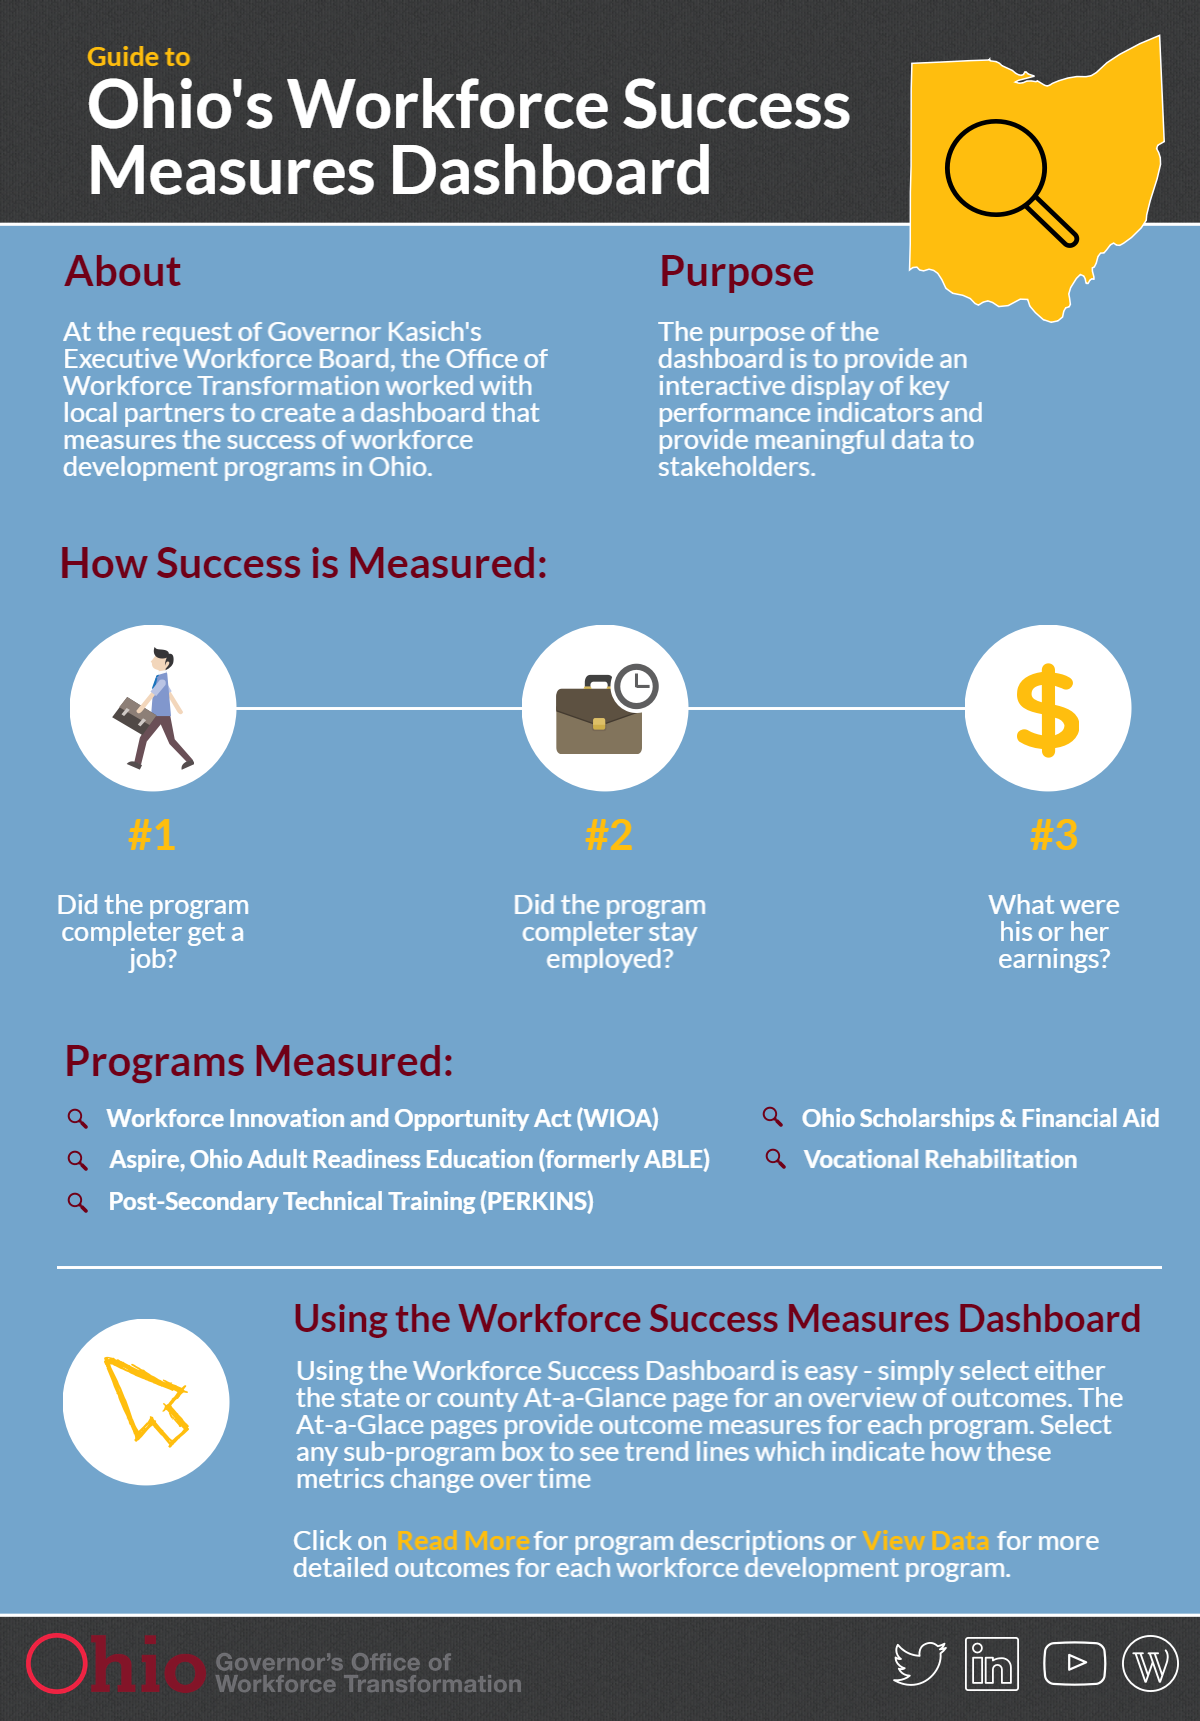
\includegraphics[width=1\linewidth]{./figures/olda_appendixb}

